\section{Exercise 08: Threat Modelling}

\subsection{A simple Data Flow Diagram}

\begin{figure}[H]
    \centering
    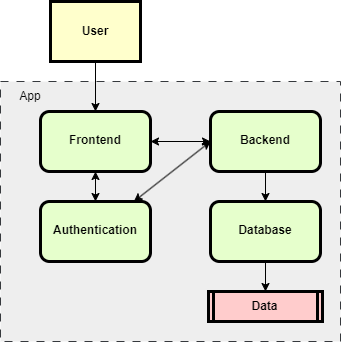
\includegraphics[width=0.5\linewidth]{pic/Flowdiagram.png}
    \caption{Flowdiagram health-app}
    \label{fig:Flowdiagram health-app}
\end{figure}

Using the STRIDE model for security threat modeling, which includes Spoofing, Tampering, Repudiation, Information Disclosure, Denial of Service, and Elevation of Privilege, we assess the following for the given web application architecture:

\begin{itemize}
    \item \textbf{Spoofing:} Attackers could impersonate legitimate users if the Authentication service is compromised.
    \item \textbf{Tampering:} The Data could be altered if the communication between the Backend and Database is not secure.
    \item \textbf{Repudiation:} Without proper logging, malicious actions could be performed without traceability.
    \item \textbf{Information Disclosure:} Sensitive data might be exposed if the Database is not adequately protected.
    \item \textbf{Denial of Service (DoS):} The App could be made unavailable if the Backend or Frontend are overwhelmed with traffic.
    \item \textbf{Elevation of Privilege:} Attackers could gain unauthorized privileges if there are vulnerabilities in the Authentication process.
\end{itemize}

To ensure robust security, each component should be fortified against these potential threats.

\subsection{Updated Flow Diagram \& STRIDE}

\begin{figure}[H]
    \centering
    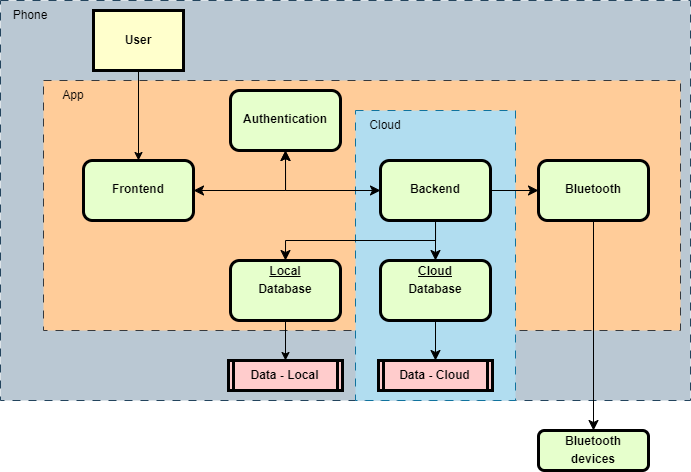
\includegraphics[width=0.9\linewidth]{pic/Flowdiagram updated.png}
    \caption{Flowdiagram updated health-app}
    \label{fig:Flowdiagram updated health-app}
\end{figure}



\begin{table}[H]
    \centering

    \begin{tabular}{ | m{4.3cm} | m{2.5cm} | m{9cm} | }
        \hline
        \rowcolor{gray!50}
        \textbf{Component}      & \textbf{Threat (STRIDE)} & \textbf{Description}                                                                  \\
        \hline
        Third-Party Devices     & Spoofing                 & Attackers could impersonate fitness devices to send false data via Bluetooth.         \\
        \hline
        Fitness Data Collection & Eavesdropping            & Unsecured Bluetooth transmission could allow interception of fitness metrics.         \\
        \hline
        Data Cleaning           & Tampering                & Malicious actors may manipulate the data cleaning process to distort fitness metrics. \\
        \hline
        Data Computation        & Repudiation              & Without proper logs, computed results could be disputed or inaccurately reported.     \\
        \hline
        Local Data Storage      & Information Disclosure   & If device security is breached, stored sensitive health data could be exposed.        \\
        \hline
        Cloud Data Storage      & Elevation of Privilege   & Inadequate access controls may lead to unauthorized data access or modifications.     \\
        \hline
    \end{tabular}
    \caption{Updated STRIDE Analysis for Fitness Tracker App}
    \label{stride-analysis}
\end{table}
This table shows the key areas of concern within the apps system that should be addressed to maintain robust security.
